\documentclass[11pt,a4paper]{article}
\usepackage[margin=23mm]{geometry}
\usepackage[T1]{fontenc}
\usepackage{lmodern}
\usepackage{hyperref}
\emergencystretch=2em
\usepackage{tikz}
\usetikzlibrary{positioning,arrows.meta}
\title{Core semantic digest: canonical coverage correction}
\date{Created-at: 2026-09-06 00:55 +02:00}
\begin{document}
\maketitle
\paragraph{Scope and current evidence.}
The user requests correction of the four reproduced defects in Core 112a254.
Prepare the exact patch against the clean audit base ae068b9, importing only
the seven-file digest commit and correcting it. Do not import portable IDs,
robotics fixtures or their corpus-golden changes. Core and provider fetched
successfully at task start. The existing audit records 18 passing original
tests and four failing identity requirements; reuse those exact negative controls.

\paragraph{Approval boundary.}
The user supplied the literal token in chat on 2026-09-06:
\texttt{APPROVED-CORE-EDIT: semantic-digest-canonical-coverage}.
Protected application and the planned verification are now authorized.
The chat turn identifier is not available. Include the token in the commit footer.

\paragraph{Owner and affected files.}
The sole implementation owner remains Core ir::semantic\_digest. Protected
application paths: \path{CORE.YAML}; \path{hymeko_core/src/ir/hash_pass.rs},
\path{mod.rs} and \path{semantic_digest.rs} in that same directory;
\path{hymeko_core/src/module_store/module_store.rs}.
Existing test owner: \path{hymeko_core/tests/unified_ir/verification/mod.rs} and
\path{semantic_digest.rs} in that same directory.
Regenerate \path{SYMBOLS.md} using the installed provider tool.
Proposal artifacts are this quartet,
\path{reports/2026-09-06-semantic-digest-correction.md} and
\path{reports/semantic-digest-correction} containing the review source,
application patch, validation log and file hashes. Extend \path{.gitattributes}
to preserve these evidence bytes. No new production dependency, IR or runner.

\paragraph{Canonical encoding.}
Keep public signatures. Build one private context from the existing path-index
owner and an ArcRec-to-first-owner-slot table. Named targets use resolved UTF-8
path segments. Canonical anonymous targets use the owner's path and the first
position in its ordered arc list. Ignore the anonymous declaration name: both
the lowerer's SymId(0) and the test builder's generated name are placeholders.
Preserve anonymous declaration annotations and parent identity.

Every ArcRec has its own domain-separated identity and full payload hash even
without a HyperArc declaration. Edges fold those hashes in slot order, preserving
duplicate references and sharing. Hash every concrete record table so reverse
dispatch omissions cannot hide record payloads. Per-declaration output stays in
DeclId order; only whole-model aggregation sorts the fixed-size hashes separately
within each record-kind domain. Counts preserve multiplicity. Values use an
iterative, order-preserving traversal with no depth truncation; preserve length,
option, sign and exact floating-point bit encodings.

Canonical mode requires unique named paths and identifiable owner slots, with
valid bindings for all anonymous declarations, at most one per ArcRec.
Otherwise use the existing explicit,
whole-model raw-ID fallback domain; hash all payloads and memberships there too.
Promise reindexing invariance only in canonical mode. Document valid symbol and
record indices as preconditions and possible panics for violations; do not claim
that bounded traversal is complete malformed-IR validation.

\paragraph{Version and preserved contracts.}
Schema stays 2; semantic algorithm version changes 1 to 2 because the encoded
bytes change. Do not keep an old-algorithm runtime selector. V1 bytes/signatures,
the deprecated Merkle body, Ir::decl\_hash, CBOR schema, parser pin, distributed
admission and the 19 existing Lean theorems remain unchanged. Rebuild any cached
V2 digest; this is not a CBOR migration. Nagare's fetched f3660cc consumer test
uses the current infallible signature; preserve that source compatibility and
run its existing merkle\_digest\_soundness family after Core approval and tests.

\paragraph{Test and resource plan.}
Before approval, check patch applicability and Rust syntax/formatting only;
these are not build or correctness results. After approval, apply in the existing
audit checkout and promote the four recorded probes into the existing test owner.
Add direct controls for anonymous placeholder/interner changes, shared identical
arcs with [A,A,B] versus [A,B,B], orphan-record payload coverage, fallback
idempotence, and depth-boundary values. Preserve the 18 incoming tests, updating
only the explicit algorithm-version assertion. Fixture setup may be consolidated
without changing any of the 29 test names, inputs, or assertions, to satisfy the
unchanged duplication baseline. Check slot/sign/weight changes
remain observable and V1 unchanged. Then run the existing complete Core gate,
CBOR corpus, admission regressions, fmt and Clippy; do not re-freeze fixture hashes.

Reuse Amaterasu's existing SDK and task-owned Core verification object store,
with an ephemeral clean source snapshot and existing cache after approval.
16 GiB memory, no extra swap, six CPUs, locked/offline tests. Record exact source,
test-only deltas, command, elapsed time and RSS/cgroup peak. A substantive fix
must pass those tests before any success claim or provider revision publication.
Worst-case storage is O(R + P + depth): R concrete/declaration records, P total
segments retained by the existing path index, and value-list nesting depth.
P can be quadratic for a deeply nested named chain; no linear-space claim is made
for arbitrary hierarchies. Record sorting costs O(R log R); encoding work also
includes all repeated target-path bytes. No performance improvement claim.
ETA: 15--25 minutes for preparation; after approval about 10--15 minutes for
implementation and bounded Core/consumer verification, based on the prior
9.7-second focused rebuild and 84-second cold Core gate plus evidence handling.

\paragraph{Rollback and acceptance.}
Before approval, rollback is only removal/reversion of the proposal artifacts.
Apply the reviewed combined patch in one coherent correction commit: the imported
algorithm 1 has four known defects and must not become a published intermediate
provider revision. The original 112a254 and proposal f35c34f preserve provenance;
reverting the correction commit restores the audit base. Revert new downstream pins before
reverting Core; recompute V2 caches for the selected algorithm version. Never
move the previous audit tag. Acceptance requires all four original counterexamples
green, new discriminating controls green, preserved V1/CBOR/admission gates and
published exact provider provenance. No main merge or release is authorized.
\begin{center}
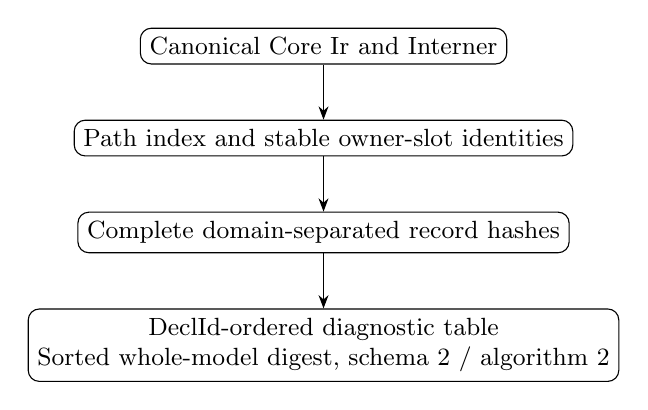
\begin{tikzpicture}[node distance=7mm,every node/.style={draw,rounded corners,align=center,font=\small},>={Stealth}]
\node (ir) {Canonical Core Ir and Interner};
\node (key) [below=of ir] {Path index and stable owner-slot identities};
\node (rec) [below=of key] {Complete domain-separated record hashes};
\node (out) [below=of rec] {DeclId-ordered diagnostic table\\Sorted whole-model digest, schema 2 / algorithm 2};
\draw[->] (ir)--(key); \draw[->] (key)--(rec); \draw[->] (rec)--(out);
\end{tikzpicture}
\end{center}

\end{document}
